
\slidesectionwithgraphic{Tree Visualization}{figures/sunburst.png}

\begin{frame}{Tree Visualization}
	\begin{columns}[T,onlytextwidth]
		\begin{column}{0.4\textwidth}
			\textbf{Tree Visualization}
			\begin{itemize}
				\setlength{\itemsep}{5pt}
				\item Visualization of tree-structured data
				\item Besides relationships of nodes, often numerical or categorical measures are of interest, too.
				\item Diverse use in information visualization
			\end{itemize}
		\end{column}   
		\begin{column}{0.6\textwidth}
			\begin{figure}
				\centering
				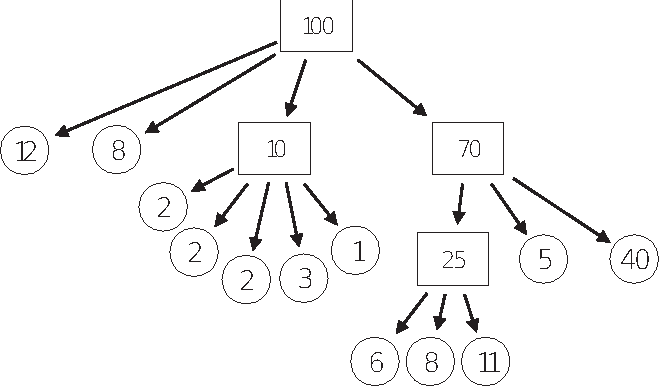
\includegraphics[width=0.9\linewidth]{images/treemap-structure}
				\caption{Example of a tree-structured dataset with associated weights for leaf nodes and accumulated weights for inner nodes.}
			\end{figure}
		\end{column}
	\end{columns}
\end{frame}

\begin{frame}{Overview of Tree Visualization Techniques}
	\begin{figure}
		\centering
		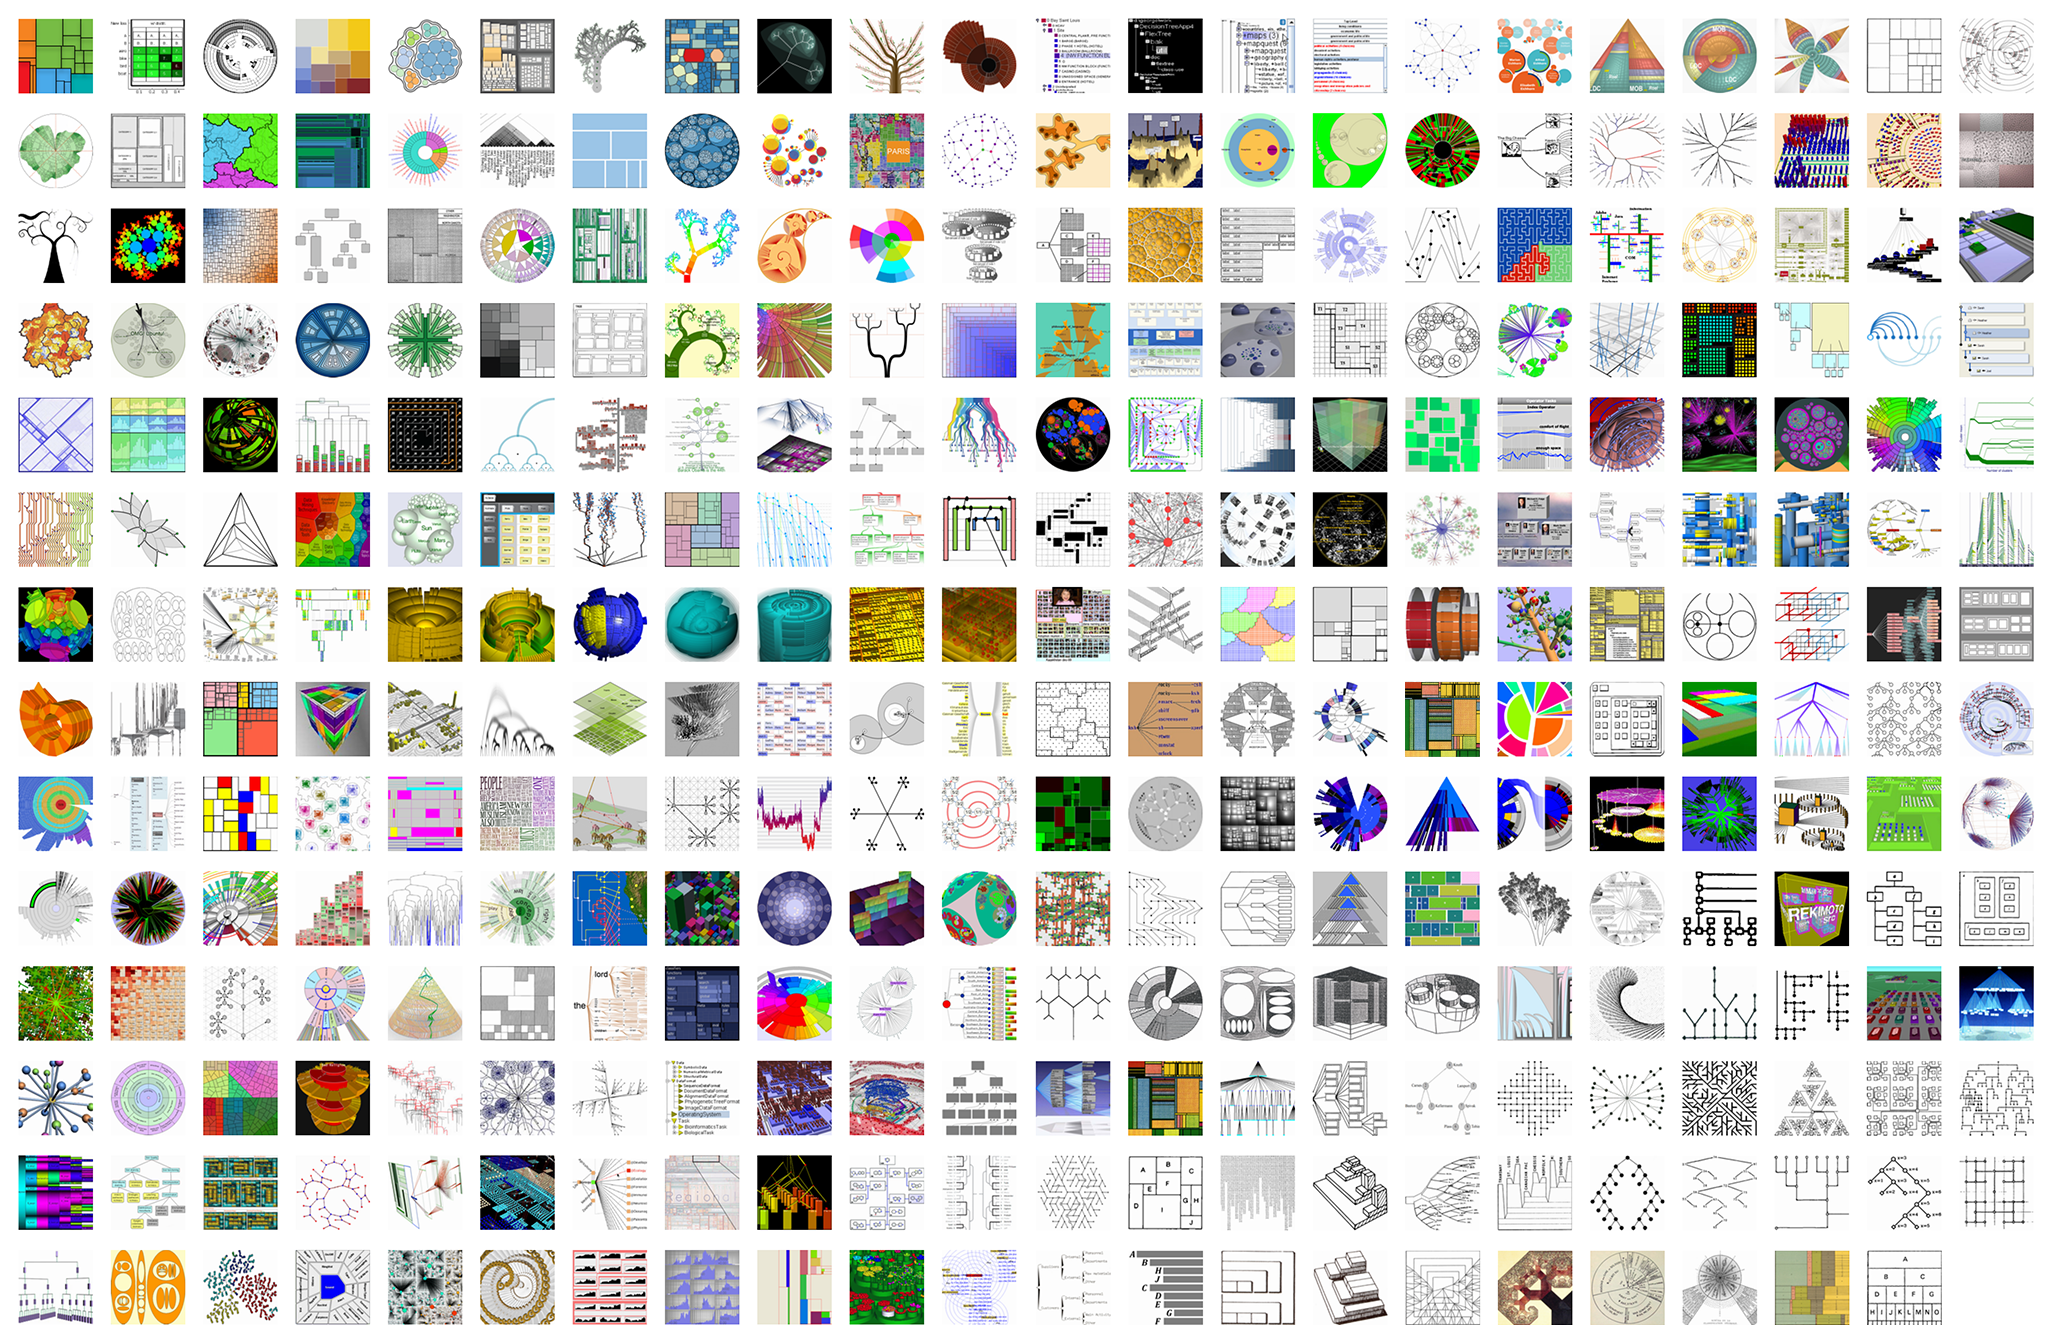
\includegraphics[width=1.0\linewidth,height=0.76\textheight,keepaspectratio]{images/treevis.net.png}
		\caption{Examples of tree visualization techniques (excerpt from \href{https://treevis.net}{treevis.net} \cite{schulz2011-treevis})}
	\end{figure}
\end{frame}

\begin{frame}{Problem Statement}
	\textbf{Problem Statement}\par
	\begin{itemize}
		\item When is a visualization technique a treemap?
		\item What are characteristics of treemaps?
		\item[]
		\pause
		\item Quick answer: it is based \enquote{on the property of containment} \cite{johnson1993-categorical}
	\end{itemize}
	\bigskip
	\bigskip
	\begin{figure}
		\centering
		\only<3|handout:1>{
% !TeX root = ../treemap-taxonomy-ivapp2020.tex

%
{%
	\footnotesize
	\centering%
	%\newlength{\definitionswidth}%
	%\newlength{\definitionsheight}%
	%\newlength{\definitionsoffset}%
	%\newlength{\definitionsimagesize}%
	%\newlength{\definitionsdescriptionsize}%
	\setlength{\definitionswidth}{\textwidth}%
	\setlength{\definitionsheight}{145pt}%
	\setlength{\definitionsoffset}{6pt}%
	\setlength{\definitionsimagesize}{0.25\definitionswidth - 2\definitionsoffset}%
	\setlength{\definitionsdescriptionsize}{0.25\definitionswidth - 0.5\definitionsoffset}%
	\begin{tikzpicture}[]
	% Images
	\node[inner sep=0,outer sep=0] (space-filling) at (-1.5\definitionsimagesize - 3\definitionsoffset, 0.5\definitionsheight) {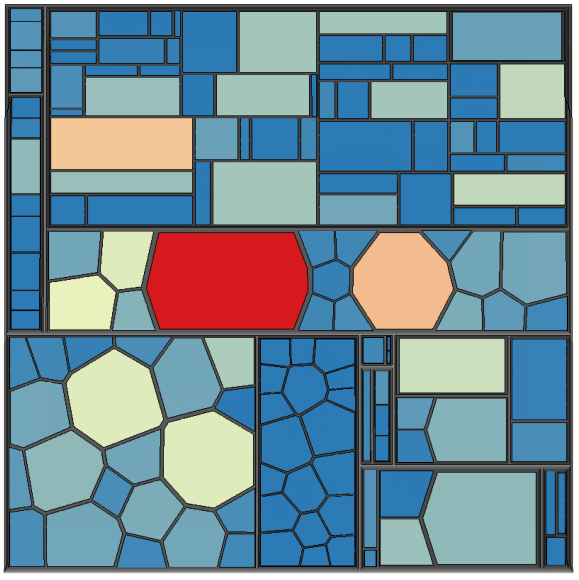
\includegraphics[width=\definitionsimagesize]{figures/mixed-treemap-layouting.png}};
	\node[inner sep=0,outer sep=0] (containment) at (-0.5\definitionsimagesize + -1\definitionsoffset, 0.5\definitionsheight) {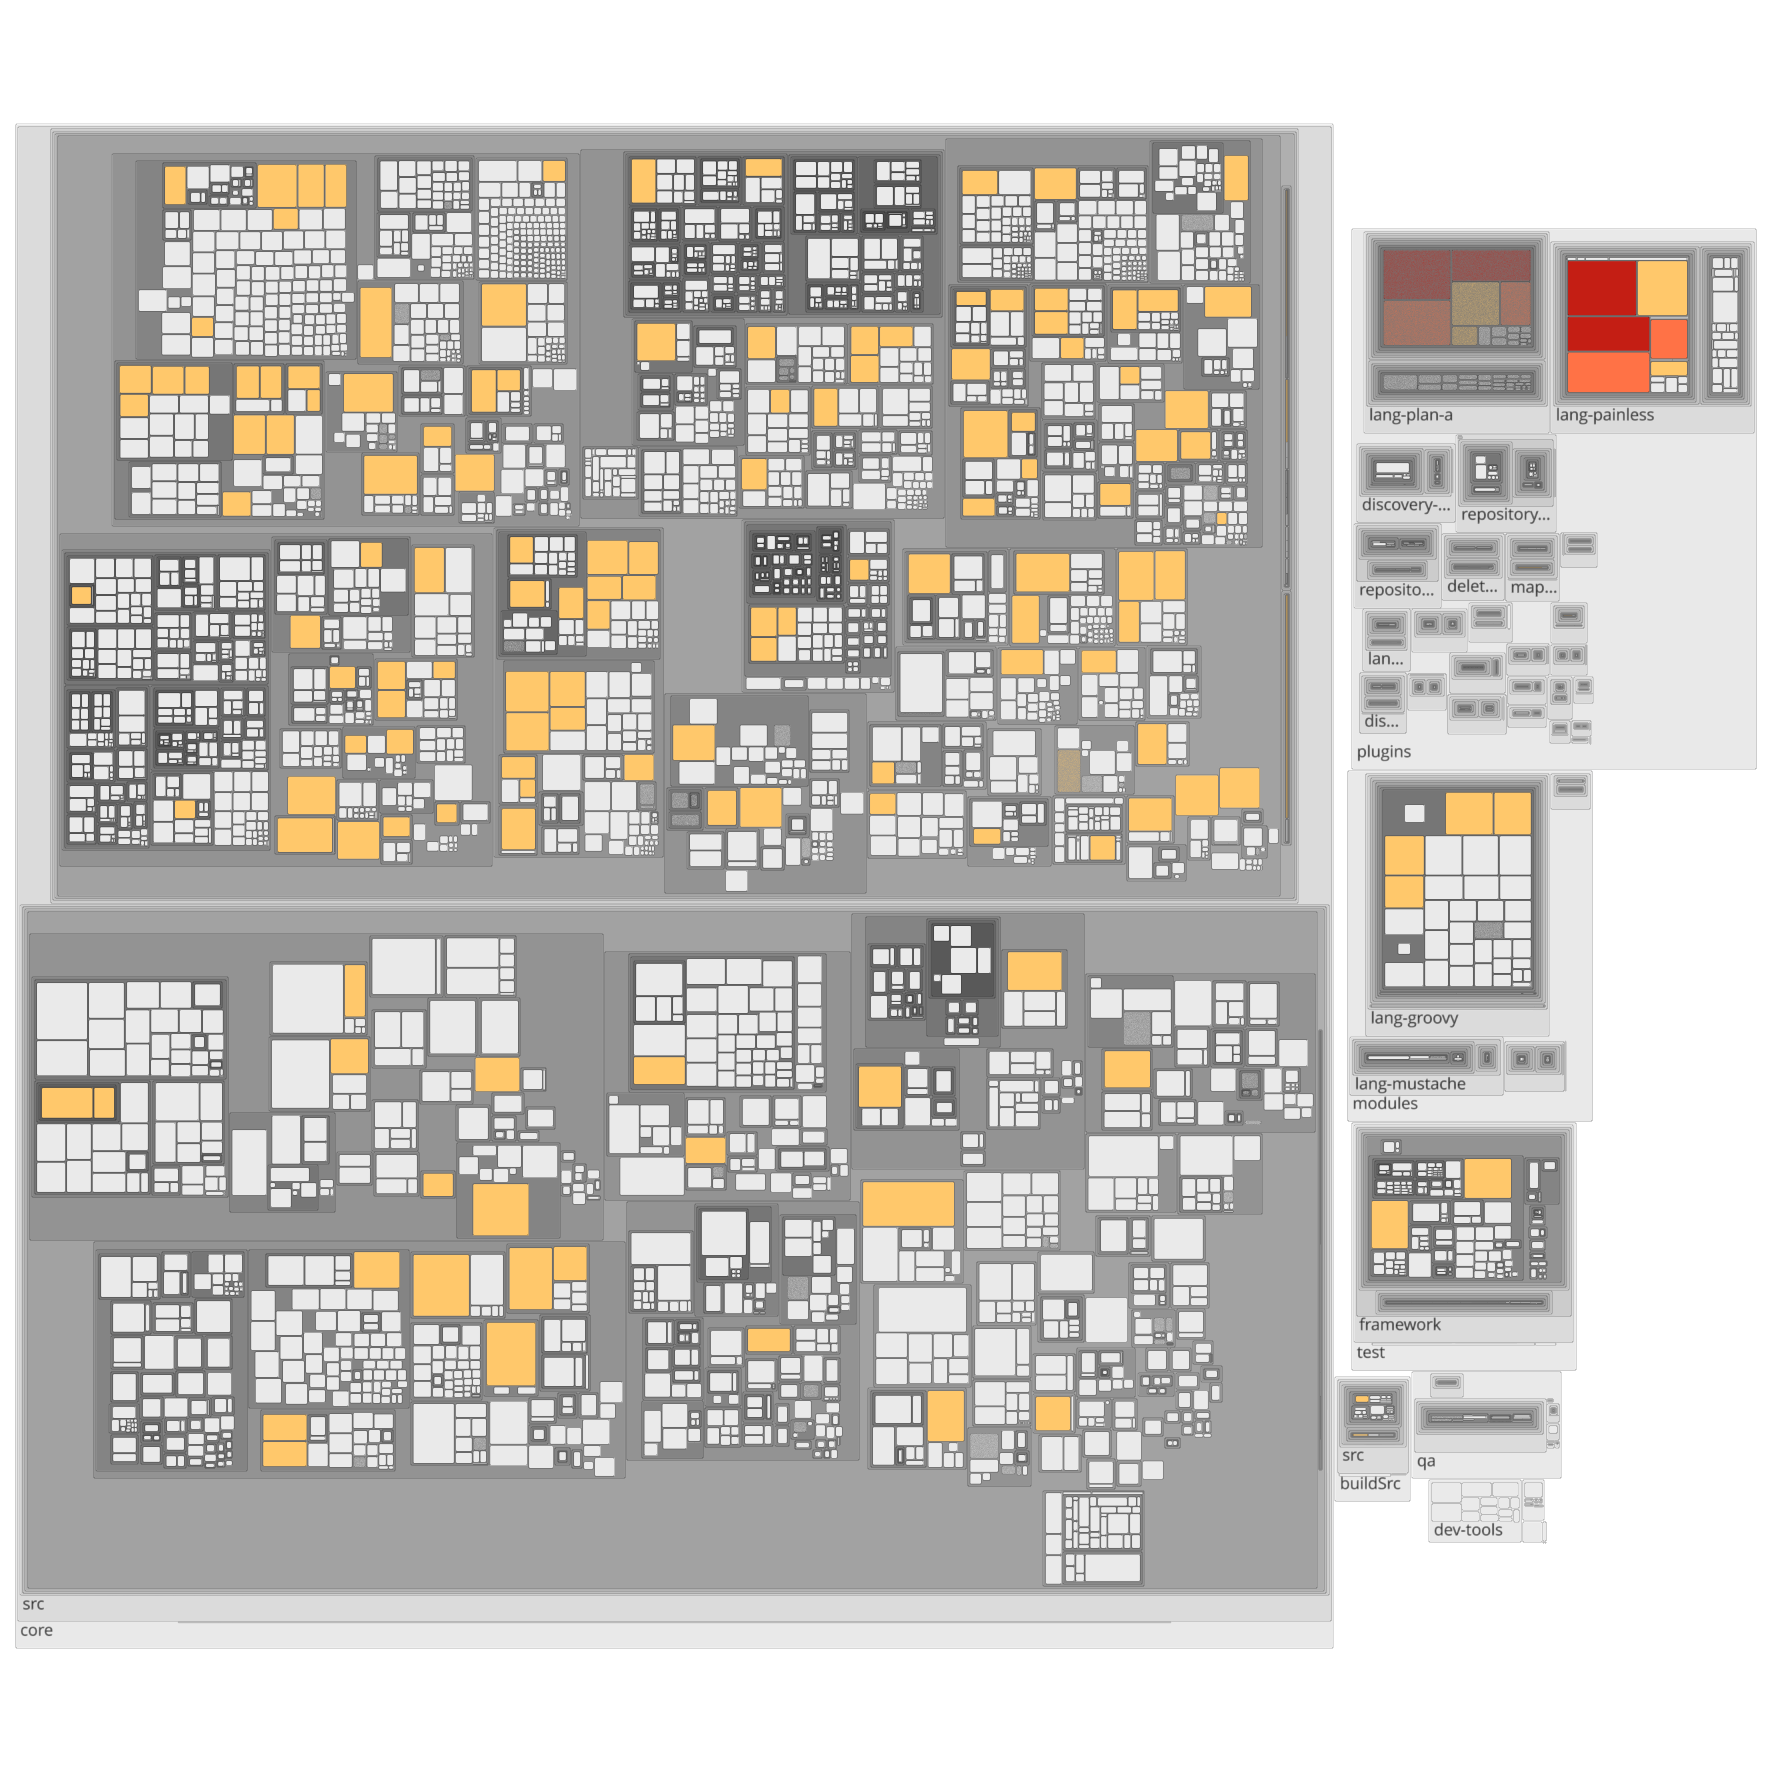
\includegraphics[width=\definitionsimagesize]{figures/evocells.png}};
	\node[inner sep=0,outer sep=0] (implicit-edge) at (0.5\definitionsimagesize + 1\definitionsoffset, 0.5\definitionsheight) {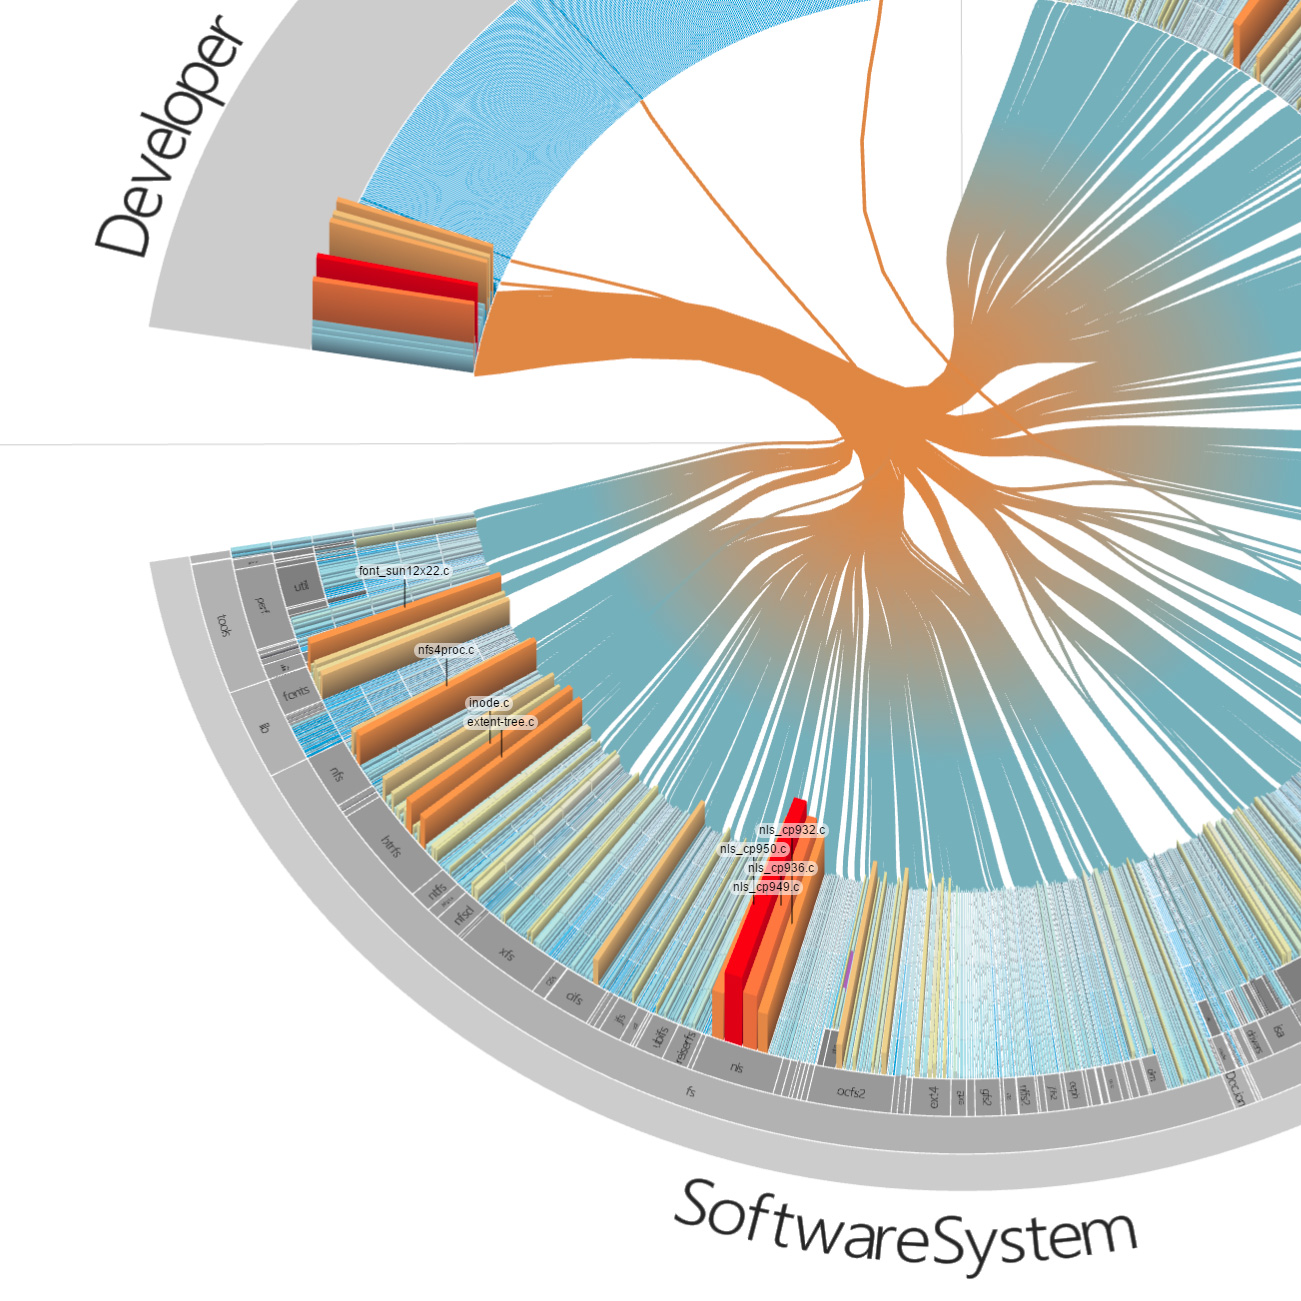
\includegraphics[width=\definitionsimagesize]{images/circular-bundle-view-bp.jpg}};
	\node[inner sep=0,outer sep=0] (mapped-tree) at (1.5\definitionsimagesize + 3\definitionsoffset, 0.5\definitionsheight) {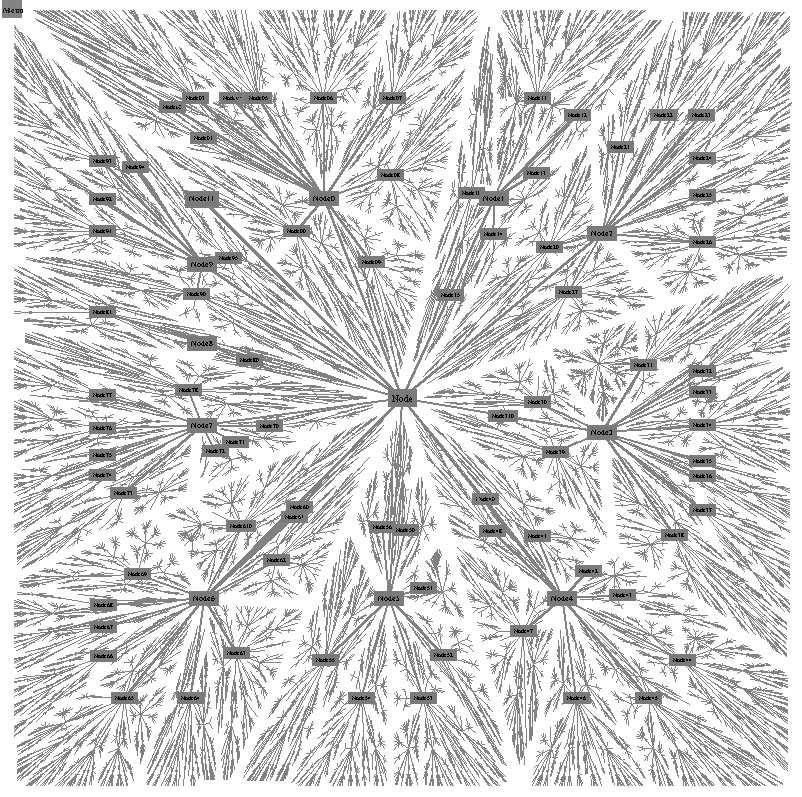
\includegraphics[width=\definitionsimagesize]{figures/spaceoptimizedtree.png}};
	\end{tikzpicture}%
}%
%
}
	\end{figure}
\end{frame}

\begin{frame}{Pipeline for Tree Visualization Techniques}
	\textbf{Tree Visualization Pipeline Model}
	\begin{itemize}
		\item Abstract model of a visualization pipeline for tree-structured data with the intend to generate tree visualizations.
		\item Important concepts are the explicit use of the topology and additional attributes for layouting and geometry processing.
	\end{itemize}
	\bigskip
	\begin{figure}
		\centering
		
% !TeX root = ../treemap-taxonomy-ivapp2020.tex

{
	\footnotesize
	%\scriptsize
	%\linespread{0.8}
    \centering
    \begin{tikzpicture}
    % Stages
    \begin{scope}[node distance = 7pt]
    \node [data] (problemdata) {};
    %
    \node [stage] (analysis) [right=of problemdata,xshift=2pt] {Analysis};
    \node [data] (visualizationdata) [right=of analysis] {};
    %
    \node [stage] (filtering) [right=of visualizationdata,text width=55pt] {Preprocessing \& Filtering};
    %
    \node [data] (focustree) [right=of filtering,yshift=10pt] {};
    \node [data] (focusdata) [right=of filtering,yshift=-10pt] {};
    %
    \node [stage] (layouting) [right=of focusdata,yshift=10pt,xshift=2pt] {Layouting};
    \node [data] (layout) [right=of layouting] {};
    
    \node [stage] (geometrycreation) [right=of layout,text width=40pt] {Geometry Creation};
    \node [data] (geometry) [right=of geometrycreation,xshift=2pt] {};
    \node [stage] (rendering) [right=of geometry] {Rendering};
    %
    \node [data] (image) [right=of rendering,xshift=2pt] {};
    \end{scope}
    % Connections
    \connectfromdata{problemdata}{analysis};
    \connecttodata{analysis}{visualizationdata};
    %
    \connectfromdata{visualizationdata}{filtering};
    \connecttodata{filtering}{focusdata};
    \connecttodata{filtering}{focustree};
    %
    \connectfromdata{focusdata}{layouting};
    \connectfromdata{focustree}{layouting};
    \connecttodata{layouting}{layout};
    %
    \connectfromdata{layout}{geometrycreation};
    \connecttodata{geometrycreation}{geometry};
    %
    \connectfromdata{geometry}{rendering};
    \connecttodata{rendering}{image};
    %
    % Labels
    %
    \node (datalabel) [above=24pt of problemdata] {};
    \node at (datalabel.west) [text depth=0pt,anchor=west,inner sep=0pt] {Problem Data};
    \draw [draw=black,very thin,shorten >= 1pt,shorten <= 3pt] (problemdata) -- (datalabel);
    %
    \node (visdatalabel) [below=10pt of visualizationdata] {};
    \node at (visdatalabel) [text depth=0pt] {Visualization Data};
    \draw [draw=black,very thin,shorten >= 1pt,shorten <= 3pt] (visualizationdata) -- (visdatalabel);
    %
    \node (treelabel) [above=14pt of focustree] {};
    \node at (treelabel) [text depth=0pt] {Topology};
    \draw [draw=black,very thin,shorten >= 1pt,shorten <= 3pt] (focustree) -- (treelabel);
    %
    \node (attributeslabel) [below=14pt of focusdata] {};
    \node at (attributeslabel) [text depth=0pt] {Attributes};
    \draw [draw=black,very thin,shorten >= 1pt,shorten <= 3pt] (focusdata) -- (attributeslabel);
    %
    \node (layoutlabel) [below=10pt of layout] {};
    \node at (layoutlabel) [text depth=0pt] {Layout};
    \draw [draw=black,very thin,shorten >= 1pt,shorten <= 3pt] (layout) -- (layoutlabel);
    %
    \node (geometrylabel) [below=24pt of geometry] {};
    \node at (geometrylabel) [text depth=0pt] {Geometry};
    \draw [draw=black,very thin,shorten >= 1pt,shorten <= 3pt] (geometry) -- (geometrylabel);
    %
    \node (imagelabel) [above=24pt of image] {};
    \node at (imagelabel.east) [text depth=0pt,anchor=east,inner sep=0pt] {Image};
    \draw [draw=black,very thin,shorten >= 1pt,shorten <= 3pt] (image) -- (imagelabel);
    %
    % Phases
    %
    \begin{scope}[on background layer]
    %
    %\node [phase,phasename=Preprocessing] (preprocessing) [fit={(analysis)(filtering)($(analysis.north)+(0pt,1.2\baselineskip)$)($(analysis.south)-(0pt,1.2\baselineskip)$)}] {};
    \node [phase,phasename=Mapping] (mapping) [fit={(layouting)(geometrycreation)($(layouting.north)+(0pt,1.2\baselineskip)$)($(layouting.south)-(0pt,1.2\baselineskip)$)}] {};
    %\node [phase,phasename=Image Synthesis] (imagesynthesis) [fit={(rendering)($(rendering.north)+(0pt,1.2\baselineskip)$)($(rendering.south)-(0pt,1.2\baselineskip)$)}] {};
    % Pipeline
    \node [pipeline] (pipeline) [fit={(analysis.west)(rendering.east)(mapping.north)(mapping.south)}] {};
    \end{scope}
    %
    \end{tikzpicture}
}

		\caption{Pipeline model for tree visualization techniques (including treemaps), adopted from \cite{santos2004-gaining}.}
	\end{figure}
\end{frame}

\slidesectionwithgraphic{Treemap}{figures/rectangular-map.png}

\begin{frame}{Treemap Visualization Technique}
	\large
	\blueify{Treemaps \cite{johnson1991-spacefilling} are used to visualize tree-structured data,}
	\bigskip
	\begin{columns}[T,onlytextwidth]
		\begin{column}{0.5\textwidth}
			\normalsize
			e.g., in demographics~\cite{jern2009-choropleth}, business intelligence~\cite{roberts2018-business}, health~\cite{chazard2006-treemaps}, and software development~\cite{merino2018-softvis}.
			\bigskip
			\begin{enumerate}
				\item non-spatial data is spatialized -- it is given a gestalt that preserves the data's structure, e.g., rectangular treemaps use nested rectangles to depict nodes,
				\item and data (attributes) are mapped to visual variables, i.e., properties of the rectangles (size and color),
				\item using one or multiple metaphors for value encoding \cite{limberger2019-softwaremaps}
			\end{enumerate}
		\end{column}
		\begin{column}{0.5\textwidth}
			\centering
			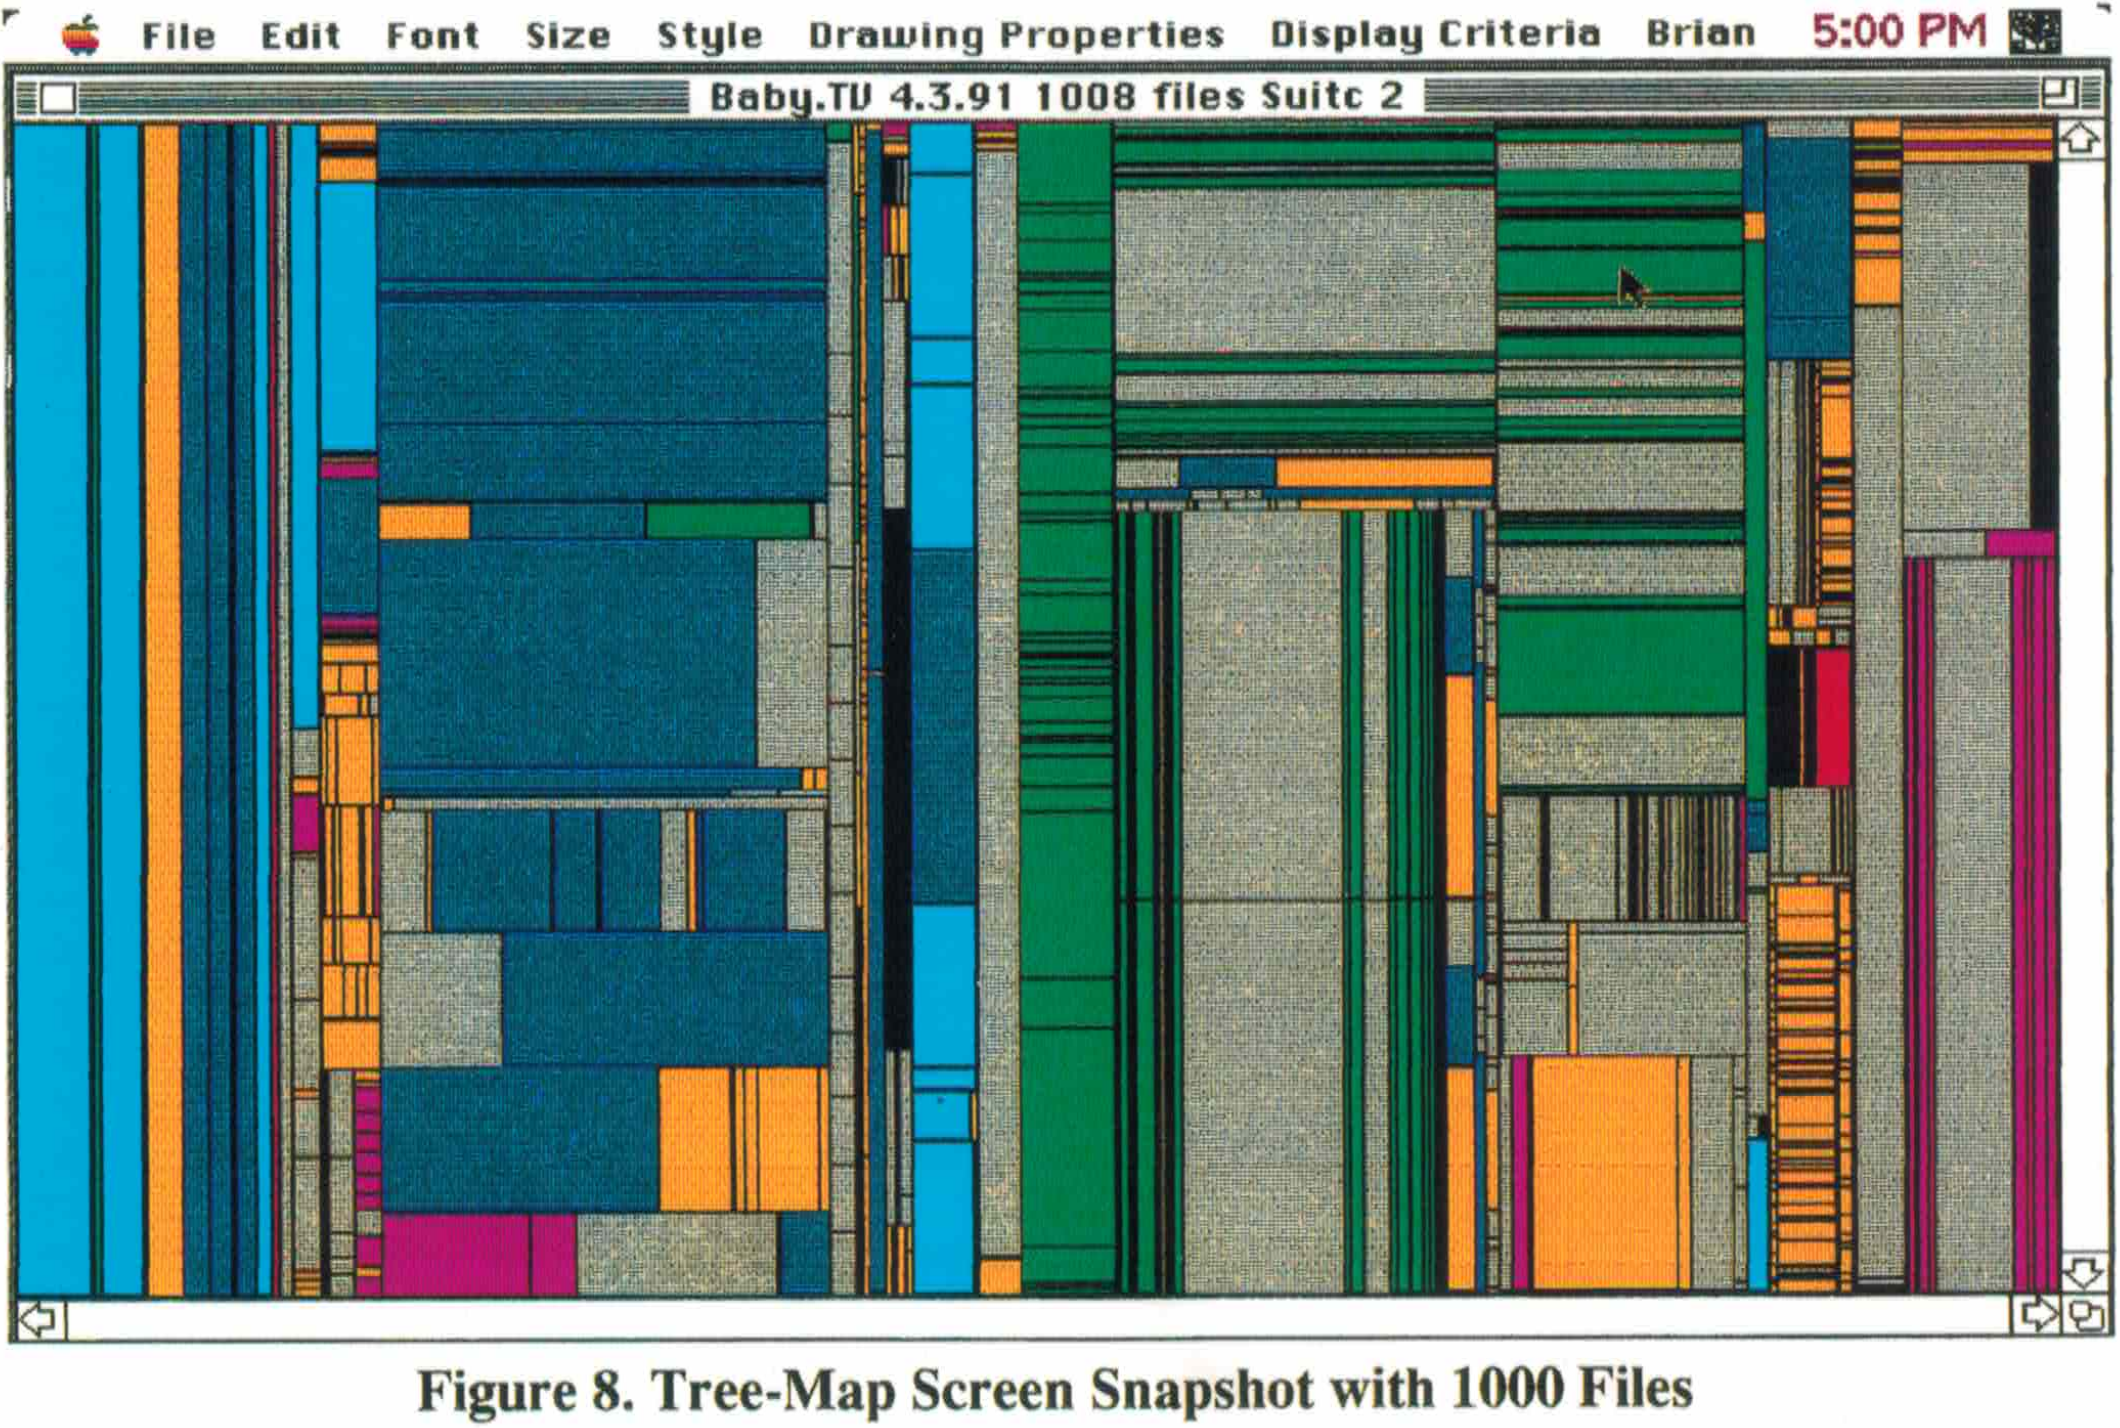
\includegraphics[width=0.9\linewidth]{images/treemap-old.png}
		\end{column}
	\end{columns}
\end{frame}

\begin{frame}{Treemap Characteristics}
	\begin{columns}[T,onlytextwidth]
		\begin{column}{0.5\textwidth}
			\textbf{Characteristics of a Treemap}\par
			\medskip
			A visualization technique is called a treemap, especially if:
			\begin{enumerate}
				\setlength{\itemsep}{5pt}
				\item A treemap is a visualization technique suitable to depict tree-structured data.
				\item There is a representation of the parent-child relationships without use of explicit edge links, i.e.,
				the containment metaphor \cite{schulz2011-implicit}.
				\item The depiction of leaf nodes implies an area or
				volume in the geometry space \cite{park2018-atomgrammar}.
				\item The representation of sibling nodes should be guaranteed to be non-overlapping \cite{johnson1991-spacefilling}.
			\end{enumerate}
		\end{column}
		\begin{column}{0.5\textwidth}
			\centering
			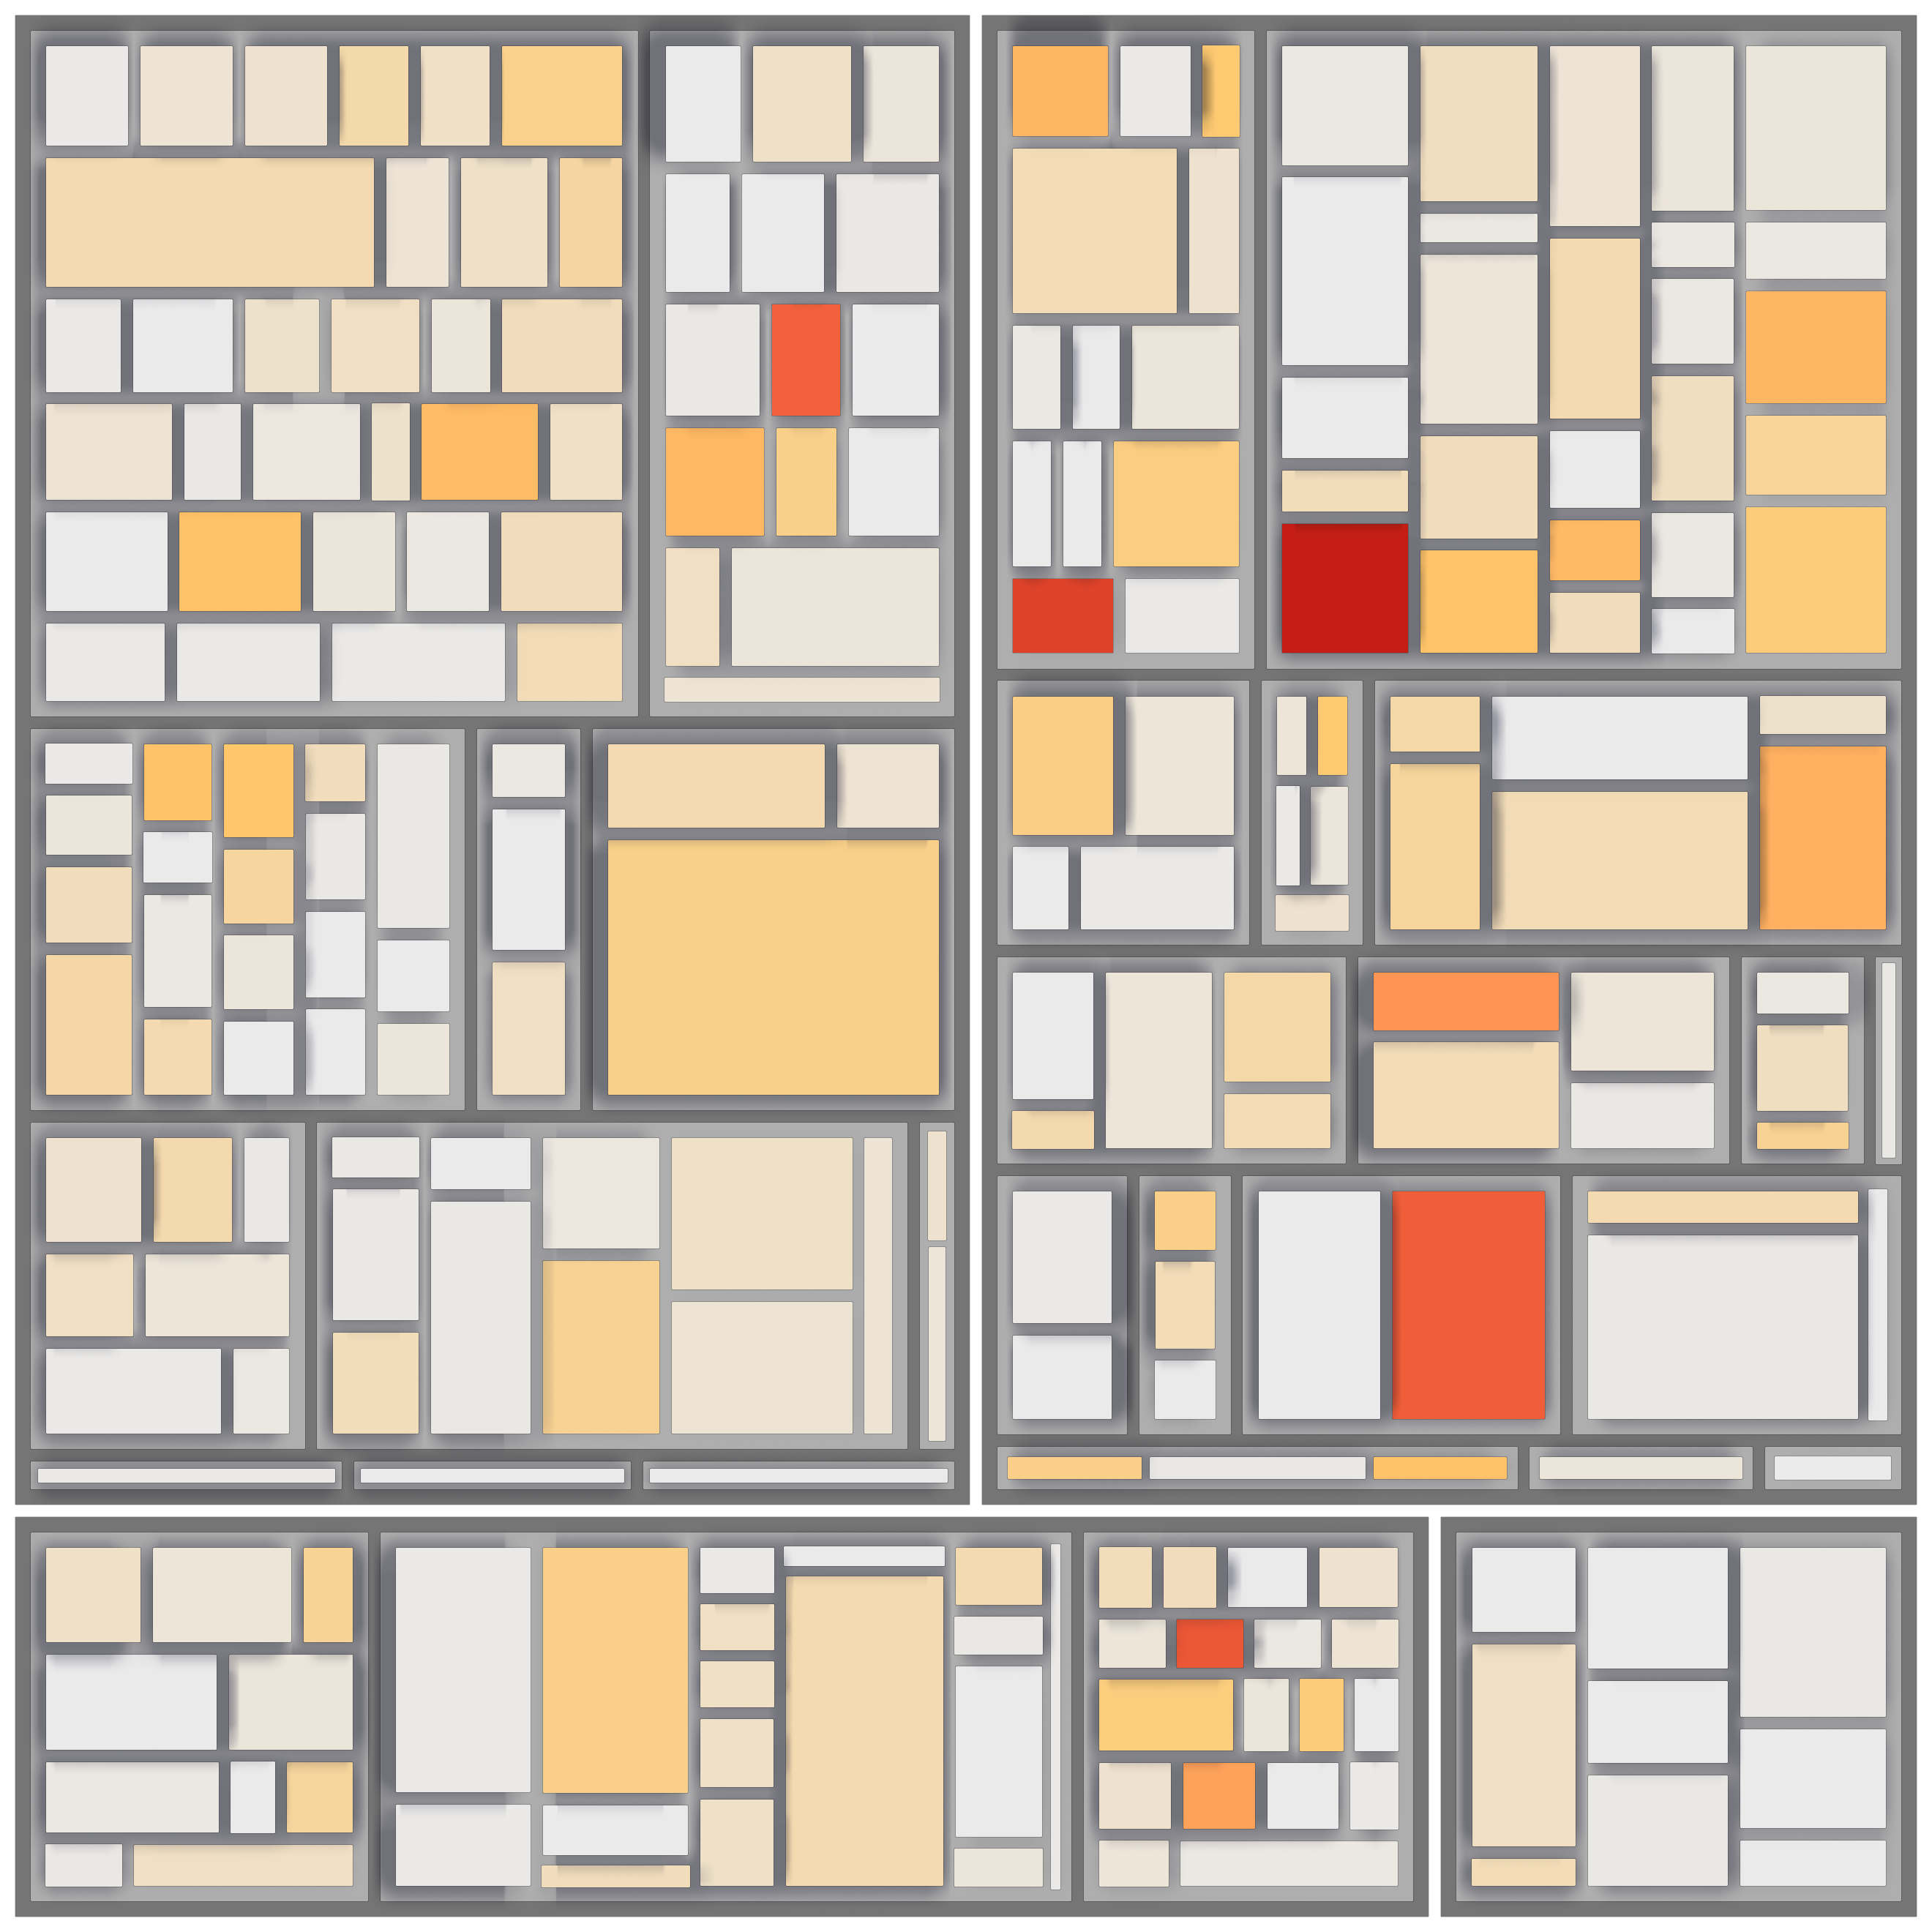
\includegraphics[width=0.9\linewidth]{images/tierpark-color.png}
		\end{column}
	\end{columns}
\end{frame}

\begin{frame}{Treemap Layouting Example}
	\textbf{Basic Treemap Layout Example}\par
	Leaf nodes are colored and have numerical weights, which can represent any associated attribute, e.g., file size.
	The weight of a parent node is defined by the sum of the weights of its child nodes.
	\bigskip
	\begin{columns}[t]
	\begin{column}{0.47\textwidth}
		\centering
		\blueify{Simple Graph}
	\end{column}
	\begin{column}{0.47\textwidth}
		\centering
		\blueify{Rectangular Treemap}
	\end{column}
	\end{columns}
	\medskip
	\centering
	\only<1|handout:0>{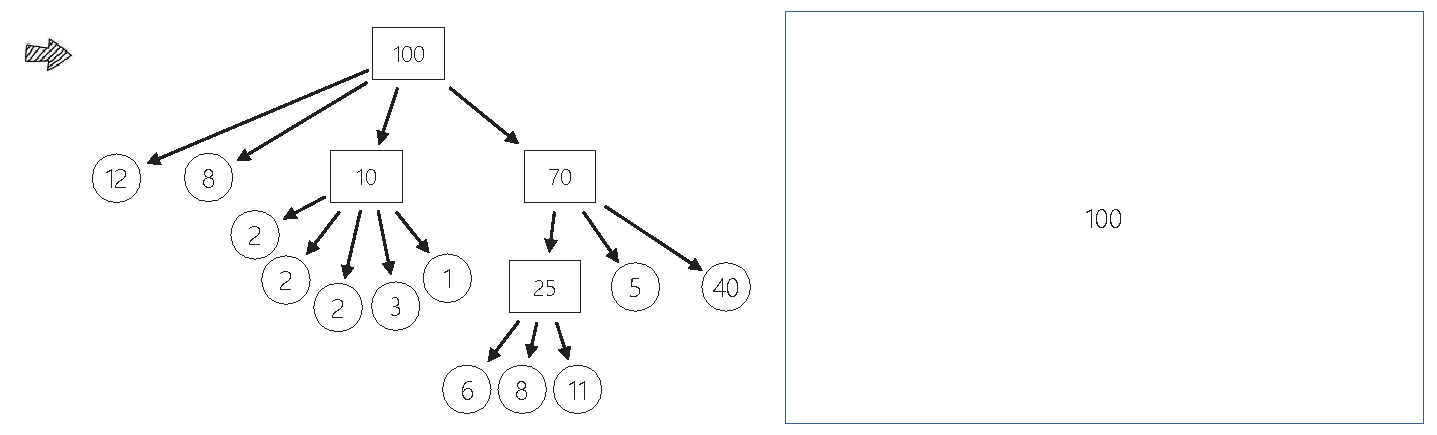
\includegraphics[width=\textwidth]{images/treemap-create-1}}
	\only<2|handout:0>{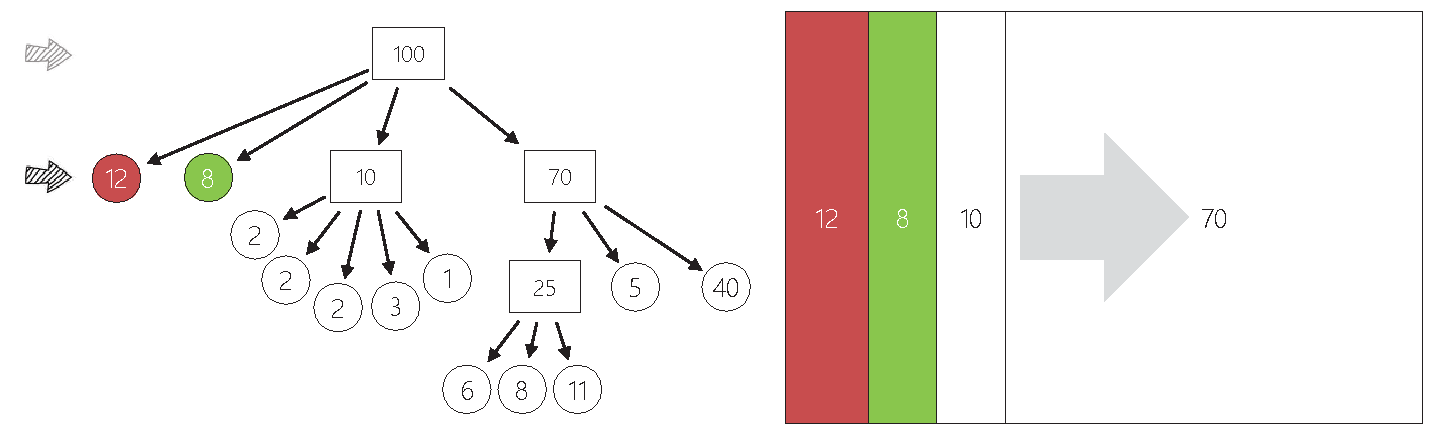
\includegraphics[width=\textwidth]{images/treemap-create-2}}
	\only<3|handout:0>{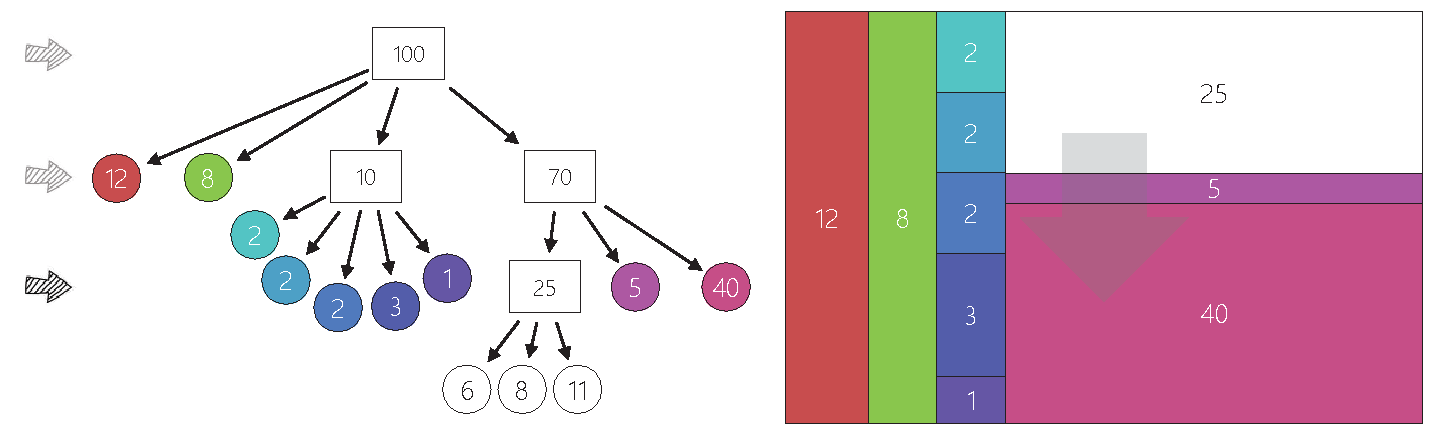
\includegraphics[width=\textwidth]{images/treemap-create-3}}
	\only<4|handout:0>{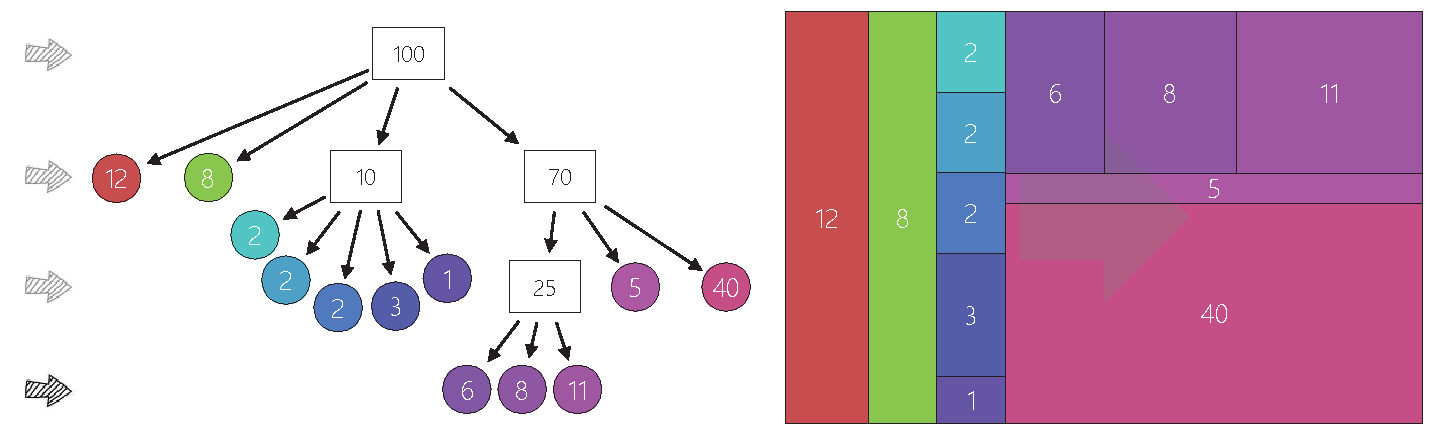
\includegraphics[width=\textwidth]{images/treemap-create-4}}
	\only<5>{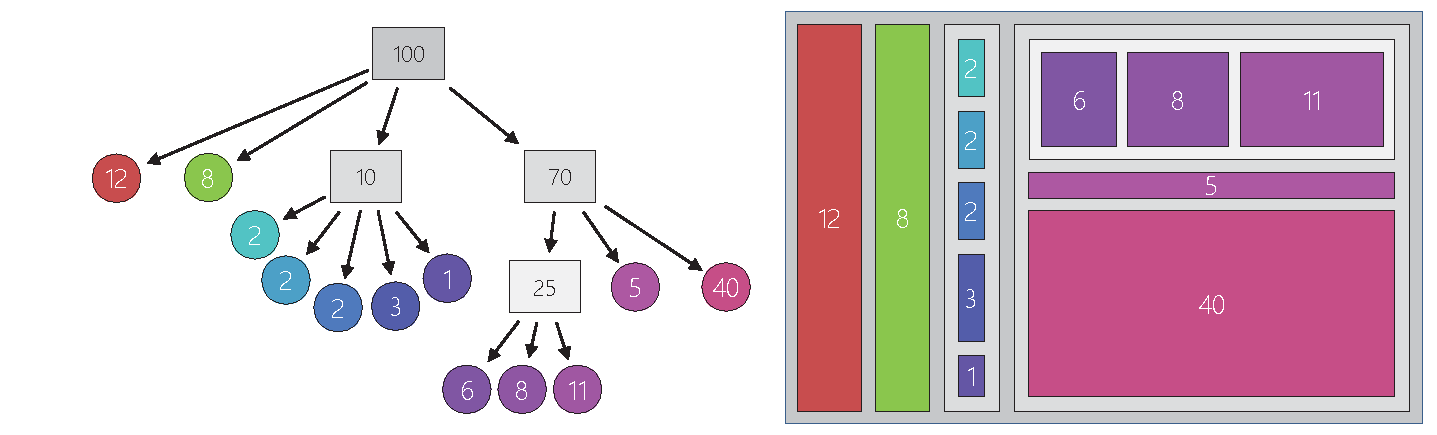
\includegraphics[width=\textwidth]{images/treemap-create-5}}
\end{frame}
